\chapter{Numerical examples} \label{chap:example}

In this chapter we illustrate the...
%
\begin{table}[h!]
	\caption{Scenarios definition.}
	\centering
	\begin{tabular}{*{6}{c}}
		\specialrule{1.5pt}{2pt}{2pt}
			\multicolumn{2}{c}{}& \multicolumn{3}{c}{Risk parameters} & Restriction \\
			\multicolumn{2}{c}{}& \multicolumn{3}{c}{$t = 1,2, \dotsc, 20$} & \textit{(R\$)} \\
	 	\specialrule{0.3pt}{2pt}{2pt}
			Scenario & Problem applied	& $\nu(t)$	& $\xi(t)$	& $\beta(t)$	&  $\alpha$ \\
		\specialrule{0.3pt}{2pt}{2pt}
			A		 & $PU(\nu,\xi)$			& 1.0		& 1.0		& -				& - \\
			B		 & $PC(\nu,\beta,\alpha)$	& 1.0		& -			& 1.0			& 50.0 \\
			C		 & $PC(\nu,\beta,\alpha)$	& 1.0		& -			& 1.0			& 20.0 \\
			D		 & $PC(\nu,\beta,\alpha)$	& 1.0		& -			& 1.0			& 0.1 \\
		\specialrule{1.5pt}{2pt}{2pt}
	\end{tabular}
	\source{Author.}
	\label{tab:scenarios}
\end{table}

%
\begin{figure} [h!]
	\caption{System's output for all scenarios.}
	\centering
	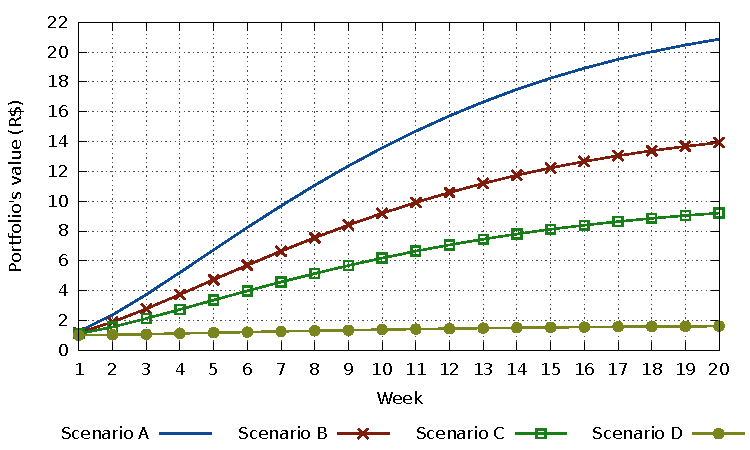
\includegraphics[width=6in,keepaspectratio]{figures/y_t}
	\source{Author.}
	\label{fig:output}
\end{figure}